\documentclass[border=10pt]{standalone}
\usepackage{tikz}
\usetikzlibrary{positioning, arrows.meta, backgrounds, fit}

\begin{document}
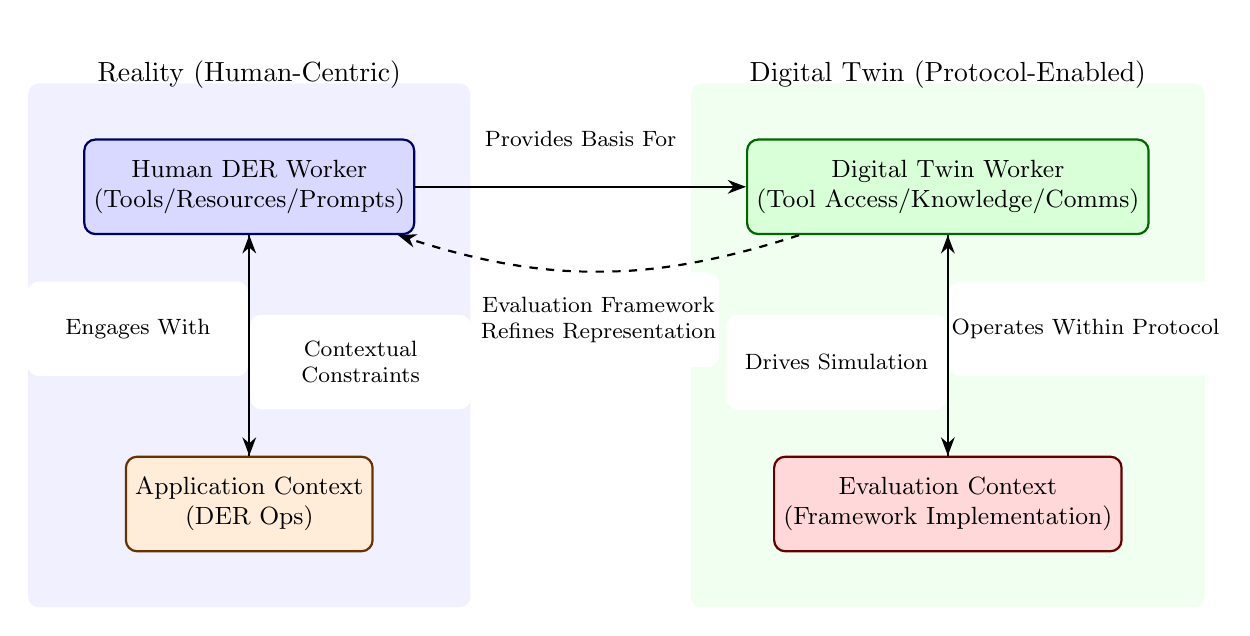
\begin{tikzpicture}[
    node distance=2.8cm and 4.2cm,
    every node/.style={rounded corners, minimum width=2.8cm, minimum height=1.2cm, align=center, font=\small},
    human/.style={fill=blue!15, draw=blue!40!black, thick},
    context/.style={fill=orange!15, draw=orange!40!black, thick},
    twin/.style={fill=green!15, draw=green!40!black, thick},
    eval/.style={fill=red!15, draw=red!40!black, thick},
    arrow/.style={-Stealth, thick},
    dasharrow/.style={-Stealth, thick, dashed},
    edgelabel/.style={font=\footnotesize, fill=white, inner sep=1pt}
]

% Human Context (left column)
\node[human] (HEW) {Human DER Worker\\(Tools/Resources/Prompts)};
\node[context, below=of HEW] (AC) {Application Context\\(DER Ops)};

% Digital Twin System (right column)
\node[twin, right=of HEW] (DT) {Digital Twin Worker\\(Tool Access/Knowledge/Comms)};
\node[eval, below=of DT] (EC) {Evaluation Context\\(Framework Implementation)};

% Human context arrows
\draw[arrow] (HEW) -- node[edgelabel, left, yshift=6pt] {Engages With} (AC);
\draw[arrow] (AC) -- node[edgelabel, right, yshift=-6pt] {Contextual\\Constraints} (HEW);

% Digital twin arrows
\draw[arrow] (DT) -- node[edgelabel, right, yshift=6pt] {Operates Within Protocol} (EC);
\draw[arrow] (EC) -- node[edgelabel, left, yshift=-6pt] {Drives Simulation} (DT);

% Core relationships (horizontal)
\draw[arrow] (HEW) -- node[edgelabel, above] {Provides Basis For} (DT);
\draw[dasharrow] (DT) to[bend left=18] node[edgelabel, below] {Evaluation Framework\\Refines Representation} (HEW);

% Subgraph backgrounds for clarity
\begin{pgfonlayer}{background}
    \node[fill=blue!6, inner sep=0.7cm, rounded corners, fit=(HEW) (AC)] {};
    \node[fill=green!6, inner sep=0.7cm, rounded corners, fit=(DT) (EC)] {};
\end{pgfonlayer}

% Titles above each subgraph
\node[font=\normalsize, above=0.2cm of HEW] {Reality (Human-Centric)};
\node[font=\normalsize, above=0.2cm of DT] {Digital Twin (Protocol-Enabled)};

\end{tikzpicture}
\end{document}
